%\documentclass[10.5pt,twocolumn]{jsarticle}
\documentclass[twocolumn]{jsarticle}

%
%コメント外に全角スペースを入れるともれなくクラッシュします.
%

%これを使って,@を記号ではなく文字として認識させます. \makeatotherで閉じます.
\makeatletter
%全く使っていませんが,一応残しておきます.
\renewcommand\subsection{\@startsection {subsection}{1}{\z@}%
{0.1\Cvs}{0.0\Cvs}
{\gt\fontsize{10.5pt}{0cm}}} %\フォントの種類,本文参照\fontsize{11pt}{0cm}#2\par}

%数字の有無がシビアだったので,partとsectionの組み合わせでやっています.
\renewcommand\section{\@startsection {section}{1}{\z@}%
{0.1\Cvs}{0.0\Cvs} %{上方向の空白\Cvs}{下方向の空白\Cvs}
{\gt\fontsize{11pt}{0cm}}} %\フォントの種類,本文参照\fontsize{11pt}{0cm}#2\par}

\renewcommand\part{%
  \setcounter{section}{0} %関数の中でもきちんと関数呼び出しができる.これを呼び出さないと,sectionが連続したものになってしまい整合性が取れなくなります..
  \if@noskipsec \leavevmode \fi
  \par\addvspace{2ex} %上方向の空白ex 単位はわかりません.
  \@afterindenttrue
  \secdef\@part\@spart}
\def\@part[#1]#2{%
  \ifnum \c@secnumdepth >\m@ne
    \refstepcounter{part}%
    \addcontentsline{toc}{part}{%
       \prepartname\thepart\postpartname\hspace{1zw}#1}%
  \else
    \addcontentsline{toc}{part}{#1}%
  \fi
  \markboth{}{}%
  {\parindent\z@\raggedright
   \interlinepenalty\@M\normalfont
   \ifnum \c@secnumdepth >\m@ne
     \gt\fontsize{11pt}{0cm} %\フォントの種類,本文参照\fontsize{11pt}{0cm}#2\par}
     \par\nobreak
   \fi
   \gt\fontsize{11pt}{0cm}#2\par} %\フォントの種類,本文参照\fontsize{11pt}{0cm}#2\par}
  \nobreak\vskip0ex\@afterheading} %vskip 下方向の空白ex 単位はわかりません.

 \makeatother




  \usepackage{graphicx}
  \usepackage[dvipdfmx]{color}
  \usepackage{url}
  \pagestyle{empty}
  %\usepackage{titlesec}

  \setlength { \textwidth } { 46zw } %1行あたり40文字,これは余白指定より前にやる必要があります
  \setlength { \textheight } { 38zw } %1枚あたり38行,これは余白指定より前にやる必要があります.
  \usepackage [top=25.4truemm, bottom=25.4truemm, left=19truemm, right=19truemm] {geometry} %余白の設定
  \renewcommand{\abstractname}{要旨} %abstractが概要と表示されるので,要旨に置き換えています.


%maketitle以前のものは,maketitleコマンドごといじる必要があり分量がとんでもないことになるので,各自以下を参考に改造してしてください.
\title{\fontsize{14pt}{0cm}\gt %\title{\fontsize{14pt}{0cm}\フォントの種類本文参照 タイトル}
高三総合人間科 \LaTeX テンプレートファイル}
\author{\fontsize{12pt}{0cm}\mc
名大附 花子}
\date{}

\begin{document}


\begin{abstract} %abstractのサイズを規定に合わせています.
{\mc\fontsize{9pt}{0cm}\
This \LaTeX\ template is released into the public domain by the copyright holders. I dedicate this \LaTeX\ template to all people who are lazy.

}\end{abstract}
% ここでmaketitle
\maketitle

\part{序論 研究課題について}

\section{研究の背景}
\LaTeX とは,一部の大学生などの熱心な学生が使っている文書作成用のソフトウェアで,WordやPagesより難しいけど楽なものです.

\section{先行研究}
組版ソフトウェアと呼ばれるものなので,Word/Pagesのように画像をドラッグしながら文章を作成するのではなく,テキストファイルを編集して文章を作成します.直感的でなく分かりにくいですが,画像の位置を自動で決め,画像および参考文献へのジャンプ(\cite{texwiki}←こんなやつです)を全て自動で記述してくれます.そのため,画像の順序が入れ替わったりしたときに時間をかけてラベルを書き直す手間が省けます.

\section{研究課題と仮説}
このファイルを編集するだけで先生が示したであろう条件(例,タイトルのフォントはゴシック体でサイズは14pt等)が自動的に適用されるので,細部に気を散らすことなく論文が書けます.

\section{研究の目的と意義}
学習コストはほんの少し高いですが,このテンプレートファイルには論文作成において必要になるであろう要素をふんだんに詰め込んだので,一部分をコピー\&ペーストすれば大抵の論文は書けますし,Google検索や図書館を使えば画像の貼り方などの書き方はいくらでも見つかるので慣れれば簡単だと思います.しかし,表\ref{fig:styles}のような表やグラフを \LaTeX で書くとなるととても大変なので,Word/Pagesで画像を作り,文章を \LaTeX で作るのが最良だと思います.

使いたくなったら,\TeX wiki\cite{texwiki}を一通り読んでインストールしてみましょう.基本的に全てここに書いてあります.


\part{本論 調査結果と考察}
\section{調査テーマ}
Texファイルをpdfに変換するには,タイプセットという作業が必要です.正しい手順で行わないとタイプセットできないことがあります.
\TeX liveが入っていない環境を用意できなかったので分かりませんが,多分texlive.iso等を使って一通り\TeX をインストールしておく必要があると思います.

\section{調査時期と方法}
\noindent Macの場合:

\begin{itemize}
  \item \TeX Shopを使っている場合:

  preferences(コマンドキー+カンマ) → set default values → Ptex(shell script)

  これでタイプセットできるようになります.

  \item 適当なeditor + terminalを使っている場合:

  Mac\TeX がインストール済みであることが条件です.図\ref{fig:makefile}のコマンドを見てやってください.

  \begin{figure}[htbp]
   \begin{center}
    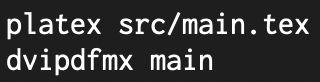
\includegraphics[width=60mm]{images/makefile.png}
   \end{center}
   \caption{コマンド}
   \label{fig:makefile}
  \end{figure}


\end{itemize}

\section{調査結果}

\noindent Windowsの場合:

\begin{itemize}
  \item \TeX Worksを使っている場合:

  少し手間がかかるので説明は\TeX wiki\cite{texwiki_work}に任せますが,説明に従って作ったpLaTeX (ptex2pdf)でタイプセットできます.

  \item VSCodeを使っている場合:

  パッケージインストールで,\LaTeX\ language supportをインストールしたのちに,powerlineから図\ref{fig:makefile}のコマンドを実行すればタイプセットできるようになります.

  \item AtomEditorを使っている場合:

  \TeX Wiki\cite{texwiki_atom}の公式通りに\LaTeX を導入していれば全てうまくいきます.詳細はそっちを見てください.

\end{itemize}


\section{考察}
\noindent Ubuntuの場合:

詳しくは検証していませんが,UbuntuにはAtomとVSCodeがインストールできるので,Windowsとmacでのやり方を参考にすればできるはずです.


\part{結論}
\section{結論}
基本的には {\bf renewcomand}コマンドを使用して,{\tt part},{\sl section},{\sc abstract}を置き換えています.もし,フォントのサイズや種類が違う,位置をずらしたい.などがあれば,コードについているコメントを頼りに色々やってみてください


\section{今後の展望}

フォントの種類は,ざっくりと分けて図\ref{fig:styles}の通りです.サイト\cite{styles}を参考にしました.これ以外にも多分きっとあるので調べてみてください.

\begin{figure}[h]
\begin{center}
\begin{tabular}{|l|l|l|ll}
\cline{1-3}
コマンド                               & 解説    & 結果                         &  &  \\ \cline{1-3}
\textbackslash{}rm & ローマン  & {\rm helo} &  &  \\ \cline{1-3}
\textbackslash{}bf & ボールド  & {\bf helo} &  &  \\ \cline{1-3}
\textbackslash{}it & イタリック & {\it helo} &  &  \\ \cline{1-3}
\textbackslash{}sf & サンセリフ & {\sf helo} &  &  \\ \cline{1-3}
\textbackslash{}sl & 斜体 & {\sl helo} &  &  \\ \cline{1-3}
\textbackslash{}sc & 全部大文字 & {\sc helo} &  &  \\ \cline{1-3}
\textbackslash{}tt & タイプライタ & {\tt helo} &  &  \\ \cline{1-3}
\textbackslash{}gt & ゴシック & {\gt helo} &  &  \\ \cline{1-3}
\textbackslash{}mc & 明朝 & {\mc helo} &  &  \\ \cline{1-3}
\end{tabular}
\end{center}
\caption{フォントの種類}
\label{fig:styles}
\end{figure}


\begin{thebibliography}{99}
\bibitem{texwiki} \url{https://texwiki.texjp.org}
\bibitem{texwiki_work} \url{https://texwiki.texjp.org/?TeXworks/設定}
\bibitem{texwiki_atom} \url{https://texwiki.texjp.org/?Atom}
\bibitem{styles} \url{http://www.latex-cmd.com/style/style.html}
\bibitem{math_latex} 手書きの数字を\LaTeX に変換してくれます \url{https://webdemo.myscript.com/views/math/index.html}
\bibitem{table_latex} 表を\LaTeX に変換してくれます \url{https://www.tablesgenerator.com/latex_tables#}
\end{thebibliography}

\end{document}
